\documentclass{beamer}

\usepackage{beamer_tom}
\usepackage{hyperref}
\graphicspath{{./images/}}

\usepackage{stackengine}
\usepackage{scalerel}
\usepackage{xcolor}
\newcommand\dangersign[1][2ex]{%
  \renewcommand\stacktype{L}%
  \scaleto{\stackon[1.3pt]{\color{red}$\triangle$}{\tiny\bfseries !}}{#1}%
}

\institute{INRIA Saclay}
\author{Thomas Moreau}
\title{
    Parietal Computational Resources:\\
    Storage
}

\setbeamertemplate{title page}[frame]
\def\extraLogo{}

\begin{document}

    \begin{frame}
        \titlepage
    %	\biblio{}
    \end{frame}

    \frame{
        \frametitle{\large \bf \code{\$HOME} - shared and backed up \keypoint{small scale}}

        {\Large The \code{\$HOME} folder on \code{drago*}}\\[.5em]
            \myitem{} Mounting point for a user \code{/home/parietal/\$USER}\\
            \myitem{} Around \code{800G}\\
            \myitem{} Shared on different machines (\code{drago*})\\
            \myitem{} Should limit to 10GB per user.\\[2em]

        {\Large The \code{\$HOME} folder on \code{margaret}}\\[.5em]
            \myitem{} Mounting point for a user \code{/home/parietal/\$USER}\\
            \myitem{} Around \code{4T}\\
            \myitem{} Shared with other teams.\\
            \myitem{} Hard limit to 50G per user
    }
    \frame{
        \frametitle{ \bf \code{dragostore} - large parietal drives
                    \keypoint{large scale}}

        { \bf \code{dragostore}}\\[.5em]
        \myitem{} Mounting point \code{/data/parietal/store/}\\
        \myitem{} Around \code{102T},\\[2em]

        { \bf \code{dragostore2}}\\[.5em]
        \myitem{} 2 file systems in \code{/data} (\code{140T}) and \code{/data2} (\code{100T}).\\
        \myitem{} Mounting points \code{/data/parietal/store2/} and \code{store3}\\

        \strongpoint{Both are accessible from \code{drago*} and \code{margaret}}
        \strongpoint{Most of your storage should go there}
        \vskip1em
    }

    \frame{
        \frametitle{Common architecture}

        Rational for the parietal storage in \code{STORE=/data/parietal/store*/}:\\[.5em]

        \myitem{} \parbox[t]{.8\textwidth}{
            The folder \code{\$STORE/data} contain {\bf shared datasets}.\\
            \emph{The data should not be modified and you should not store new files here, only new datasets in there original form.}
        }\\[1em]
        \myitem{} \parbox[t]{.8\textwidth}{
            The folder \code{\$STORE/derivative} contain shared derivative from the datasets.\\
            \emph{Some common preprocessing steps are very time consuming, there results are stored in this folder so they can be used by everyone in the team.}
        }\\[1em]
        \myitem{} \parbox[t]{.8\textwidth}{
            The folder \code{\$STORE/work/\$USER} contains working files.\\
            \emph{Here you can put your own files as well as cached results.}
        }\\[1em]
        \emph{{\bf Note:} On \code{margaret}, the folder \code{/scratch} can be used to store temporary files for fast access.}

    }

    \begin{frame}{Evaluating storage space on a node}

        {\Large \bf \code{df} - Disk space usage:}\\[1em]

        \myitem{} Use \code{df -h}, for human readable output.\\[.5em]

        {\centering 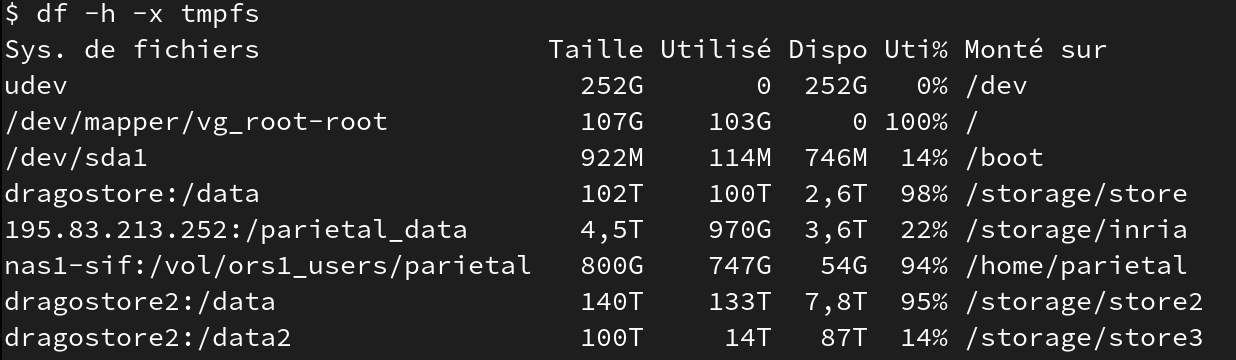
\includegraphics[width=.9\textwidth]{df.png}\\[1em]}

        \emph{use \code{-x tmpfs} to filter out some entries.}\\[1em]

        \myitem{} {\bf File sytem:} link between physical parts of a disk and "file names".\\
        \myitem{} {\bf Mounting point:} point from which "file names" are linked to part of a given disk.


    \end{frame}

    \begin{frame}{Evaluating what takes space}

        {\Large \bf \code{du} or \code{ncdu} - Folder sizes:}\\[1em]

        \myitem{} Use \code{du -h -d 1 .}, for human readable output.\\[.5em]

        {\centering 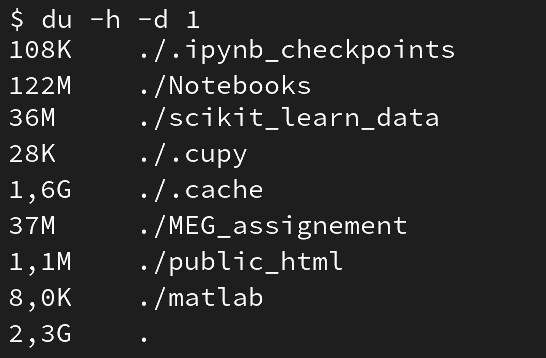
\includegraphics[width=.4\textwidth]{du.png}\\[1em]}

        \emph{Option \code{-d 1} to report up to depth 1.\\
              It takes a lot of time if your \code{\$HOME} folder is large.}\\[1em]

        \myitem{} Use \code{ncdu}  for a more interactive usage.


    \end{frame}

    \begin{frame}{Evaluating what takes space}

        {\Large \bf Using \code{pandas} - File sizes:}\\[1em]

        \myitem{} \code{ncdu} on \code{/data/parietal} takes hours\\[.5em]
        \myitem{} Lilian computed a large \code{DataFrame} with all file sizes:\\[.5em]


        \quad\quad\quad{\centering
        \begin{beamercolorbox}[rounded=true, shadow=false, wd=.7\textwidth]{title}
            \color[rgb]{0,.3,.6}\textnormal{\texttt{%
            \;df = pd.read\_parquet(\\
                \;\quad    "/data/parietal/store2/work/sysadmin"\\
                \;\quad    "/storage\_23\_10\_2021.df"\\
                \;)\\
            \;df.query(\\
            \;\quad"username == 'thmoreau'"
            \;)['size'].sum() / 1e9
            }}
    \end{beamercolorbox}}


    \end{frame}

    \begin{frame}{Lilian's report}

        {\centering
        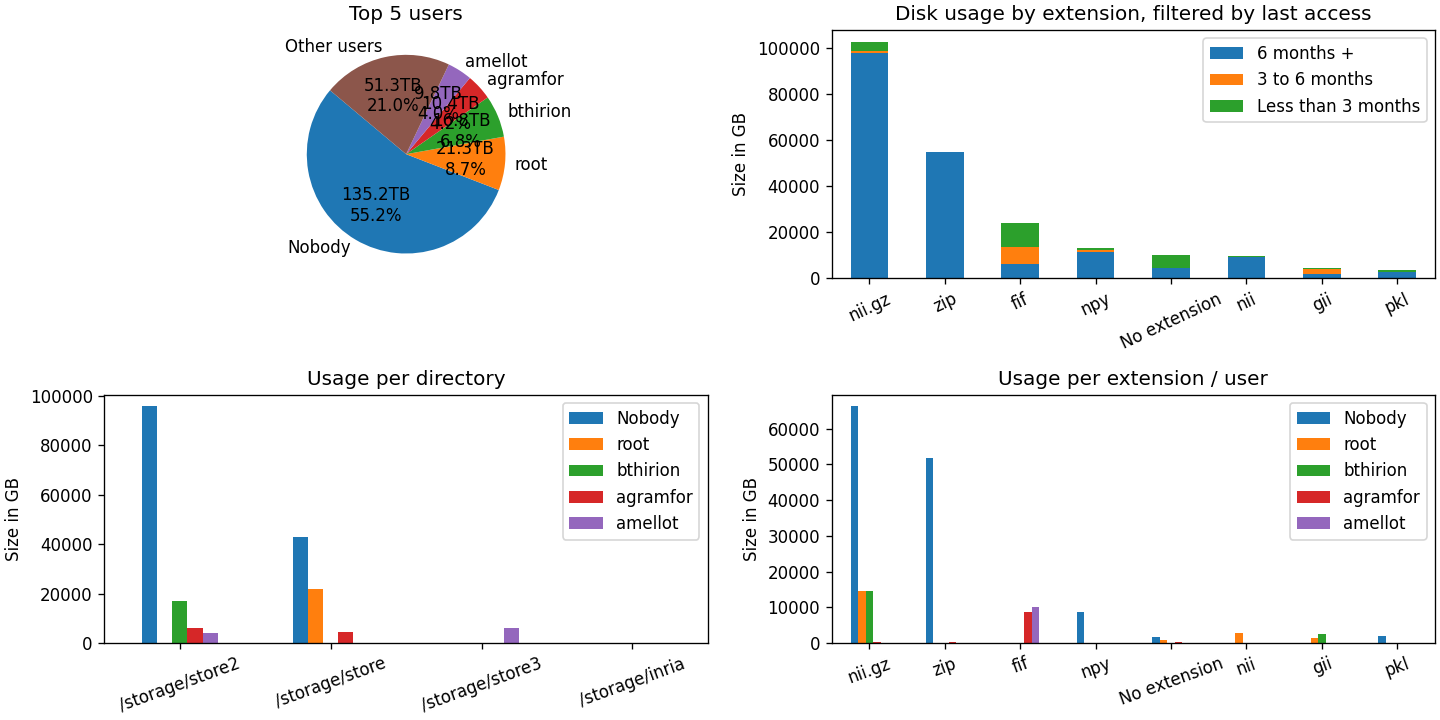
\includegraphics[width=\textwidth]{storage.png}
        }

    \end{frame}

    \begin{frame}{TODO}

        \myitem{} \parbox[t]{.9\textwidth}{run \code{ncdu} on your \code{\$HOME} folders in \code{drago} and \code{margaret} and clean big unused folders.\\[1em]}

        \myitem \parbox[t]{.9\textwidth}{Find your big joblib cache folder and clean the one that you don't need anymore.\\
        You can use Lilian's \code{DataFrame} to find them, see in the notes.\\[1em]}

        \myitem{} See list of potential tasks in \\{\centering \url{https://notes.inria.fr/VFX8bePxRJO\_78rcd9rE7A\#}.\\[1em]}


    \end{frame}

\end{document}